\section{Anexo I: Preparación del entorno de desarrollo.}

En este anexo se resumen los pasos a seguir para la puesta a punto del entorno de desarrollo, también se incluye la forma de ejecutar el flujo de trabajo y abrir la vista interactiva con el informe de resultados. En primer lugar se tiene que instalar el entorno de desarrollo Knime, la aplicación esta disponible para sistemas operativos Windows, MacOs y Linux. Se puede descargar a través de la siguiente url: \url{https://www.knime.com/downloads}

\bigbreak

Una vez instalado el entorno de desarrollo, se tiene que abrir el fichero EVAL\_MOD\_PRED.knwf incluido en el material. Es posible que en este punto se pida instalar alguna extensión en este caso se recomienda la instalación por defecto que ofrece Knime. Por último, es necesario guardar el flujo de trabajo en una ruta local.

\bigbreak

Para que funcione el proceso automático es importante crear un directorio en la misma ruta donde previamente se ha guardado el flujo de trabajo. El nombre del directorio tiene que ser DATA, hay que tener en cuenta que el nombre ha de ir en mayúsculas. Otro punto importante a la hora de ejecutar el proceso automático, es cambiar el nombre de la clase en la cabecera de los ficheros de datos, por defecto el nombre que se tiene que poner es CLASS. En el nodo CLASS NAMES, se puede modificar el nombre que se usa por defecto para la clase, este nodo situado en el flujo principal. Para finalizar, se tienen que incluir los ficheros en el directorio DATA.

\bigbreak

\begin{figure}[htp]
    \centering
    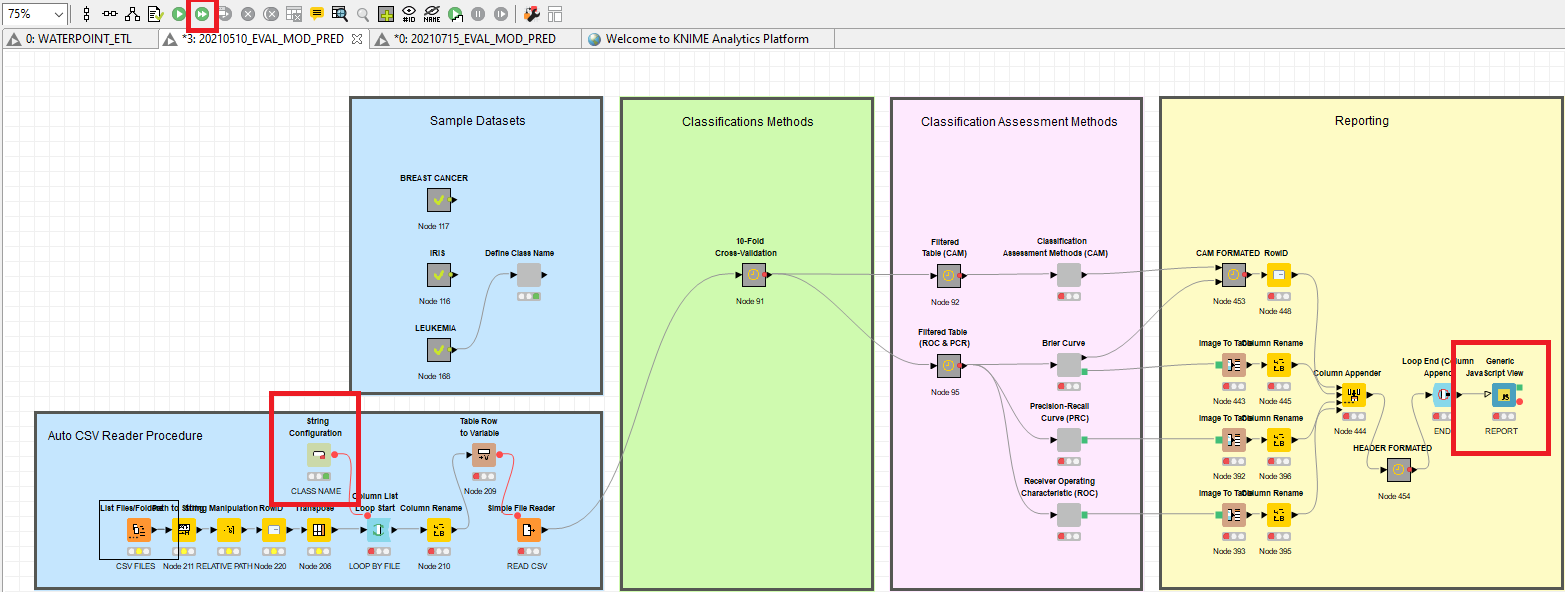
\includegraphics[scale=0.4]{config.png}
    \caption{Flujo principal, se seleccionan en rojo los componentes con los que tiene que interaccionar el usuario.}
    \label{fig:4}
\end{figure}

\bigbreak

Para la ejecución completa del flujo de trabajo, tenemos que hacer clic en el botón verde situado en la barra de herramientas. Alternativamente se puede utilizar el comando shift+F7 para ejecutar el flujo al completo. Los resultados se presentan mediante el nodo REPORT situado en el flujo principal, se puede acceder al informe haciendo clic derecho sobre el nodo y seleccionando la opción de vista interactiva.

\clearpage